\documentclass[11pt)]{beamer}
\usetheme{Copenhagen}

\defbeamertemplate*{headline}{split}
{%
  \leavevmode%
  \hbox{%
  \begin{beamercolorbox}[wd=.5\paperwidth,ht=2.65ex,dp=1.5ex,right]{section in head/foot}%
    \usebeamerfont{section in head/foot}\insertsectionhead\hspace*{2ex}
  \end{beamercolorbox}%
  \begin{beamercolorbox}[wd=.5\paperwidth,ht=2.65ex,dp=1.5ex,left]{subsection in head/foot}%
    \usebeamerfont{subsection in head/foot}\hspace*{2ex}\insertsubsectionhead
  \end{beamercolorbox}}%
  \vskip0pt%
}
\usepackage{subcaption}
\defbeamertemplate*{footline}{split}
{
	\leavevmode%
   	\hbox{%
      \begin{beamercolorbox}[wd=.5\paperwidth,ht=2.25ex,dp=1ex,center]{author in head/foot}%
        \usebeamerfont{author in head/foot}\insertshortauthor
      \end{beamercolorbox}%
      \begin{beamercolorbox}[wd=.4\paperwidth,ht=2.25ex,dp=1ex,center]{title in head/foot}%
        \usebeamerfont{title in head/foot}\insertshorttitle
      \end{beamercolorbox}%
      \begin{beamercolorbox}[wd=.1\paperwidth,ht=2.25ex,dp=1ex,right]{date in head/foot}%
        \usebeamerfont{date in head/foot}
        \insertframenumber{} / \inserttotalframenumber\hspace*{2ex}
      \end{beamercolorbox}}%
      \vskip0pt%
}

\setbeamertemplate{caption}{\raggedright\insertcaption\par}



\usepackage[utf8]{inputenc}
\usepackage{amsmath}
\usepackage{amsfonts}
\usepackage{amssymb}
\usepackage{graphicx}
\usepackage{lmodern}
\usepackage{color}
\usepackage{multirow}
\graphicspath{ {./figures/} }
\author{Judith Abécassis, Timothée Lacroix}
\title{SSL via Locally Sensitive Hashing (LSH)}
%\setbeamercovered{transparent} 
\setbeamertemplate{navigation symbols}{} 
%\logo{} 
\institute{Graphs in Machine Learning} 
\date{April 2015} 
%\subject{}
\AtBeginSection[]

\usepackage{tikz}
\usetikzlibrary{shapes,arrows,positioning}

\begin{document}
\graphicspath{{./../report/figures/}}
\begin{frame}
\titlepage
\end{frame}

{
  \begin{frame}
    \frametitle{Table of contents}
    \tableofcontents[currentsection]
  \end{frame}
}


\section{Challenge}
\begin{frame}{Classify a lot of elements in a SSL context}
  \begin{figure}
    \centering
    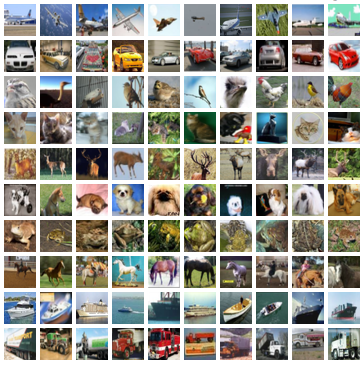
\includegraphics[width=\textwidth]{cifar-10.png}
    \caption{Crowd}
  \end{figure}
\end{frame}

\section{Semi-Supervised Learning Framework}
\begin{frame}{Leverage information from unlabeled nodes in the graph}
\begin{itemize}
 \item Labelling data is costly
 \item Unlabelled points can help us identify the underlying structure of the data
 \item Graphs are natural discretization of manifolds
 \item kNN / $\epsilon$ graph constructions lead to good estimate of the diffusion process over the manifold.
\end{itemize}
\end{frame}

\begin{frame}{The harmonic solution}
\begin{itemize}
 \item We want the labelling to be smooth over the manifold (hence over the graph).
 \item Direct solution exists but doesn't scale
 \item Can be computed iteratively with access to the Laplacian
\end{itemize}
\end{frame}
\section{Locality Sensitive Hashing}
\begin{frame}{Presentation of the principle}
\begin{itemize}
 \item Project points over a set of random directions, then quantize.
 \item Close points will stay close. Distant points will often stay distant.
 \item Sometimes two close neighbors will be on two sides of a boundary, leading to errors.
\end{itemize}
\end{frame}

\begin{frame}{Speed vs Accuracy}
\begin{itemize}
 \item The query time grows linearly with the number of points / bin.
 \item Errors become more frequent with smaller bins. 
 \item We need to find a good compromise between speed and accuracy. Some methods auto-adapt their parameters.
\end{itemize}
\end{frame}

\section{Theory}
\begin{frame}{Strategy}
\begin{itemize}
 \item Bounding $\Arrowvert L^*-\hat{L}\Arrowvert_F=\mathcal{O}(1)$ is enough to get an $O(n^{-1/2})$ term in the generalization bound.
 \item We can use the guarantees from LSH :
 $$p^w(u) = \int_0^w \frac{1}{u}\left( \frac{1}{\sqrt{2\pi}}\exp(-\frac{t^2}{2u^2})\right)\left(1-\frac{t}{w}\right)dt$$
 \item For a node $x$, a real neighbor $y$ and a wrong neighbor $z$, we need to bound : 
 $$\mathbb{E}[\Arrowvert x-y\Arrowvert_2^2 + \Arrowvert x-z\Arrowvert_2^2]$$
\end{itemize}

\end{frame}

\begin{frame}{Limitations to obtaining a bound for LSH}
$$\mathbb{E}[\Arrowvert x-y\Arrowvert_2^2 + \Arrowvert x-z\Arrowvert_2^2] = \int_y \int_z (1-P^w(y))P^w(z)dydz$$
This term depends on :
\begin{itemize}
 \item The underlying manifold $\mathcal{M}$ geometry
 \item The rate of decay of our similarity measure
 \item Density of points around $x$
\end{itemize}
\end{frame}

\begin{frame}{Empirical results on LSH accuracy}
\begin{itemize}
\item Instead of getting a theoretical bound, we have explored in a practical setting the error made by LSH
\begin{figure}[!h]
 \begin{subfigure}{0.27\textwidth}
   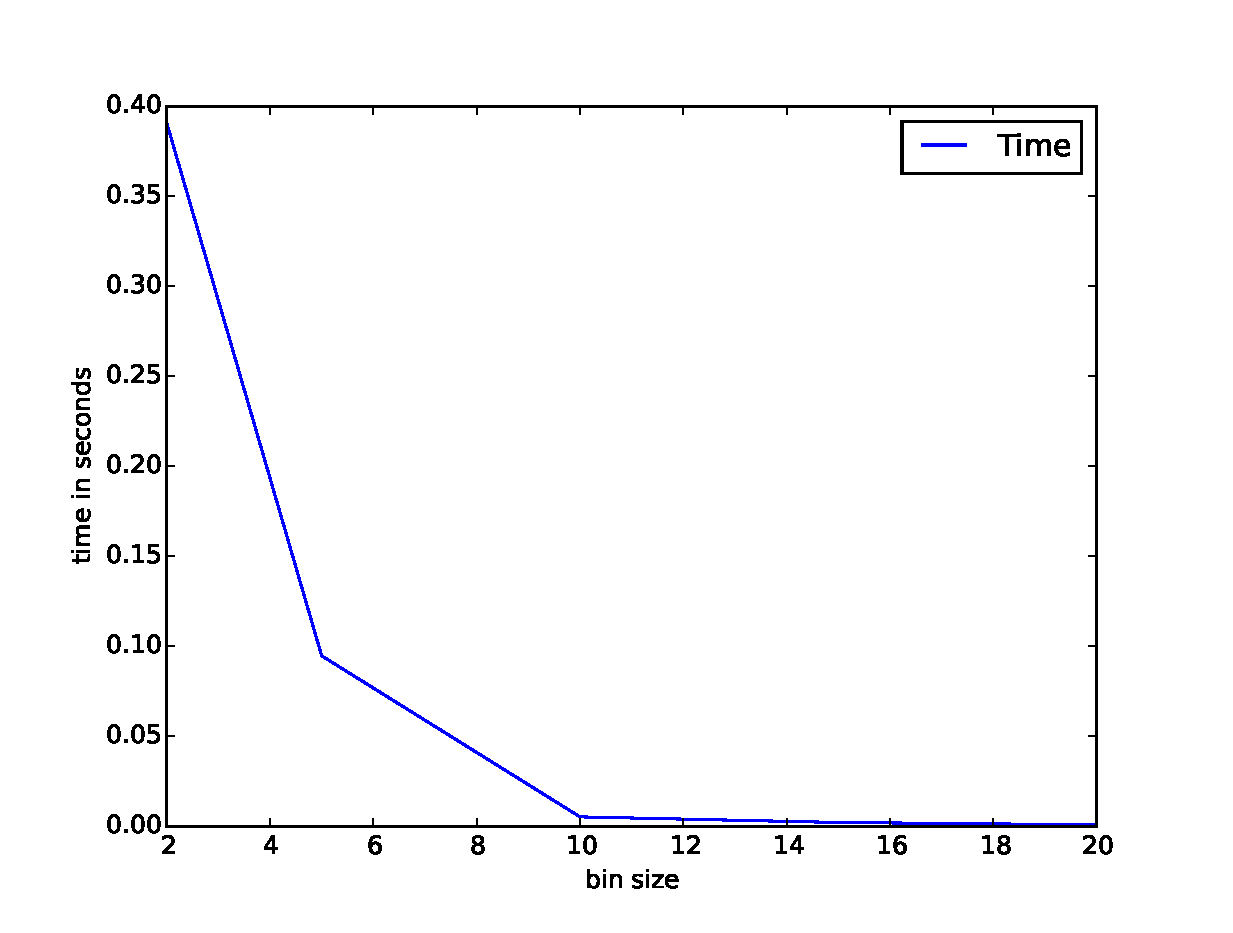
\includegraphics[width=\textwidth]{time_binsize.eps}
   \caption{Average time for a nearest neighbor query, as the number of bucket increases}
 \end{subfigure}\hfill
 \begin{subfigure}{0.27\textwidth}
   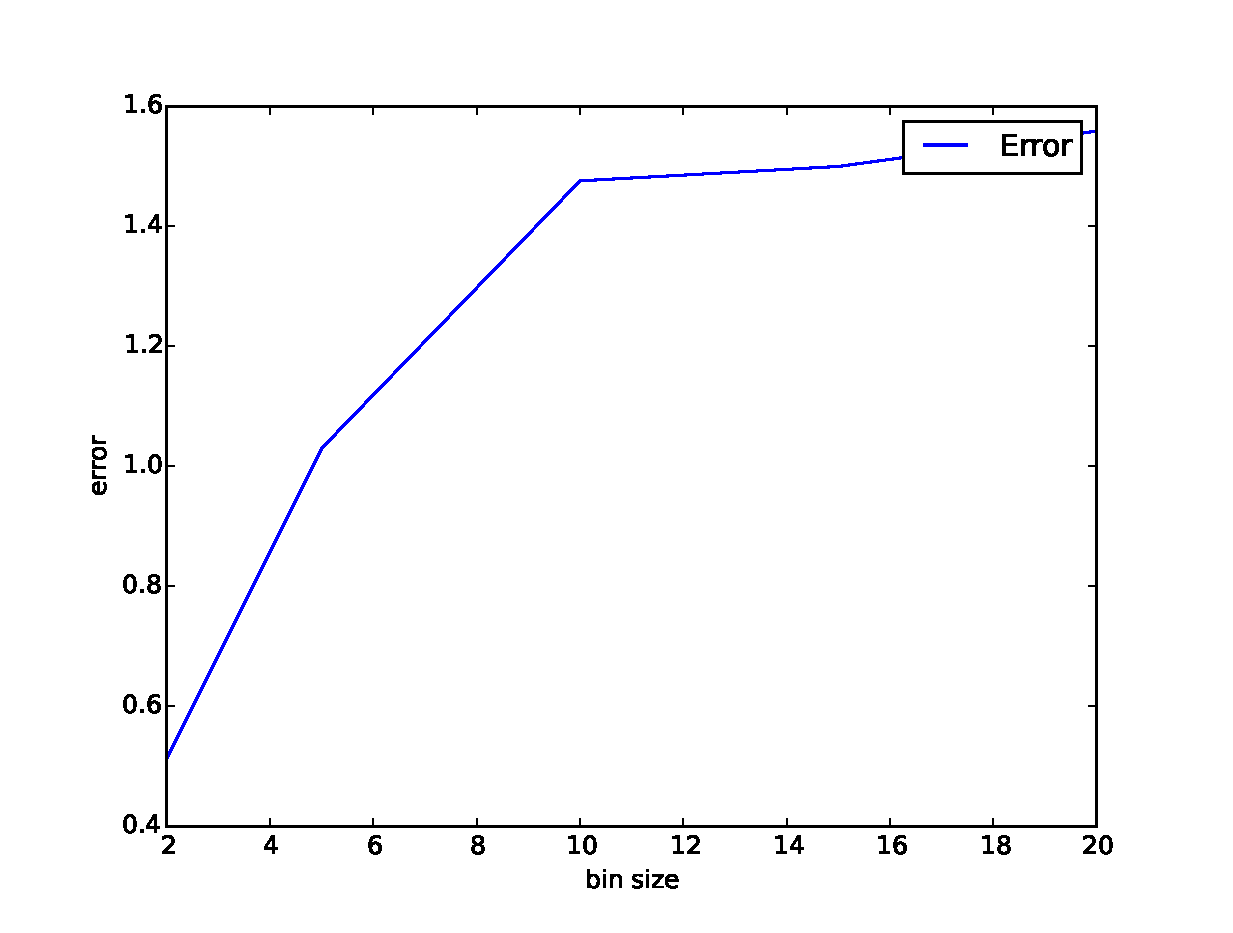
\includegraphics[width=\textwidth]{error_binsize.eps}
   \caption{Average normalized error for an approximated line of the Laplacian and an exact line, as the number of bucket increases}
 \end{subfigure}\hfill
 \centering
 \begin{subfigure}{0.27\textwidth}
   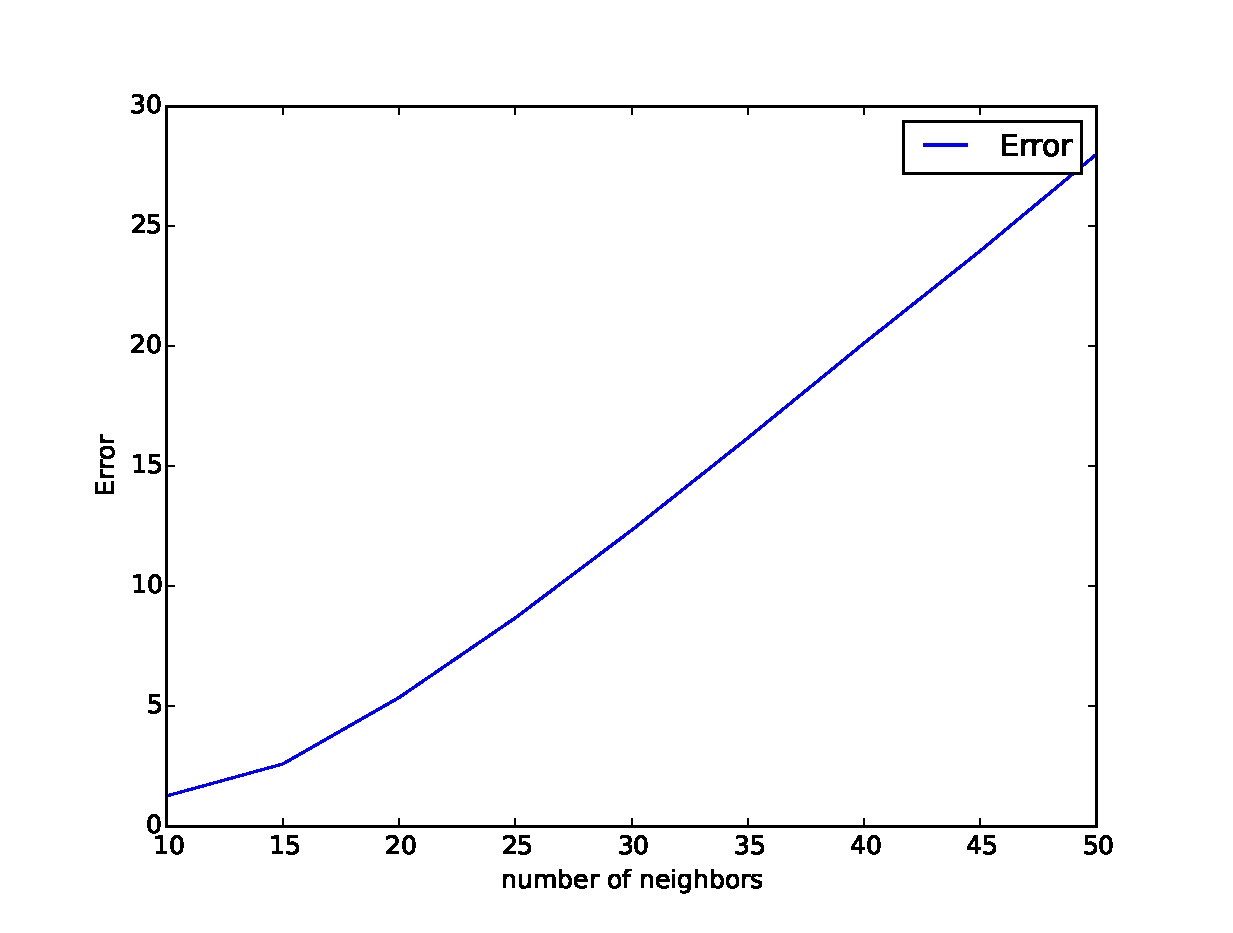
\includegraphics[width=\textwidth]{error_k.eps}
   \caption{Average normalized error for an approximated line of the Laplacian and an exact line, as the number of neighbor increases}
 \end{subfigure}

\end{figure}
\end{itemize}

\end{frame}

\section{Experiments}
\begin{frame}{The tinyImage dataset and preprocessing steps}
\begin{itemize}
\item ~80 million unlabeled images
\item CIFAR-100 labels: 10 classes with 600 labeled images in each
\item enriched with GIST descriptors (384 dimensions)
\item PCA on the 80M images: down to 32 dimensions
\end{itemize}
\end{frame}

\begin{frame}{Setting to assess performance}
\begin{itemize}
\item we consider $C$=10 random classes
\item for each class, we select $t$ positive and $t$ negative (in one of the remaining $100-C$ classes, $t\in \{0, 1, 2, 3, 5, 8, 10, 16, 20, 40, 60, 100\}$. Those are labeled nodes from the training set.
\item we compute the lerning step (by LSH+HFS or Fergus algorithm)
\item we select 100 positive test images and 200 negative ones for each of the $C$ classes (unlabeled)
\item we measure precision at 15 \% recall.
\end{itemize}
\end{frame}

\begin{frame}{Problems with LSH and Graphlab implementations}
We have encountered several issued due to computation time while applying LSH+HFS method
\begin{itemize}
\item computation of the graph is long (~2600 sec)
\item one propagation step is long too (~1100 sec)
\end{itemize}
We have adapted the setting to save some computation time
\begin{itemize}
\item only positive and neutral labels (0 and 1s), to allow doing one propagation for the $C$ classes and not $C$ propagation steps
\item only consider the first 25 classes, and not 100 (otherwise it is even longer)
\end{itemize}

{\color{red}\textbf{Problem} results are no longer comparable to the Fergus baseline}

\end{frame}

\begin{frame}{Results}
\begin{figure}
  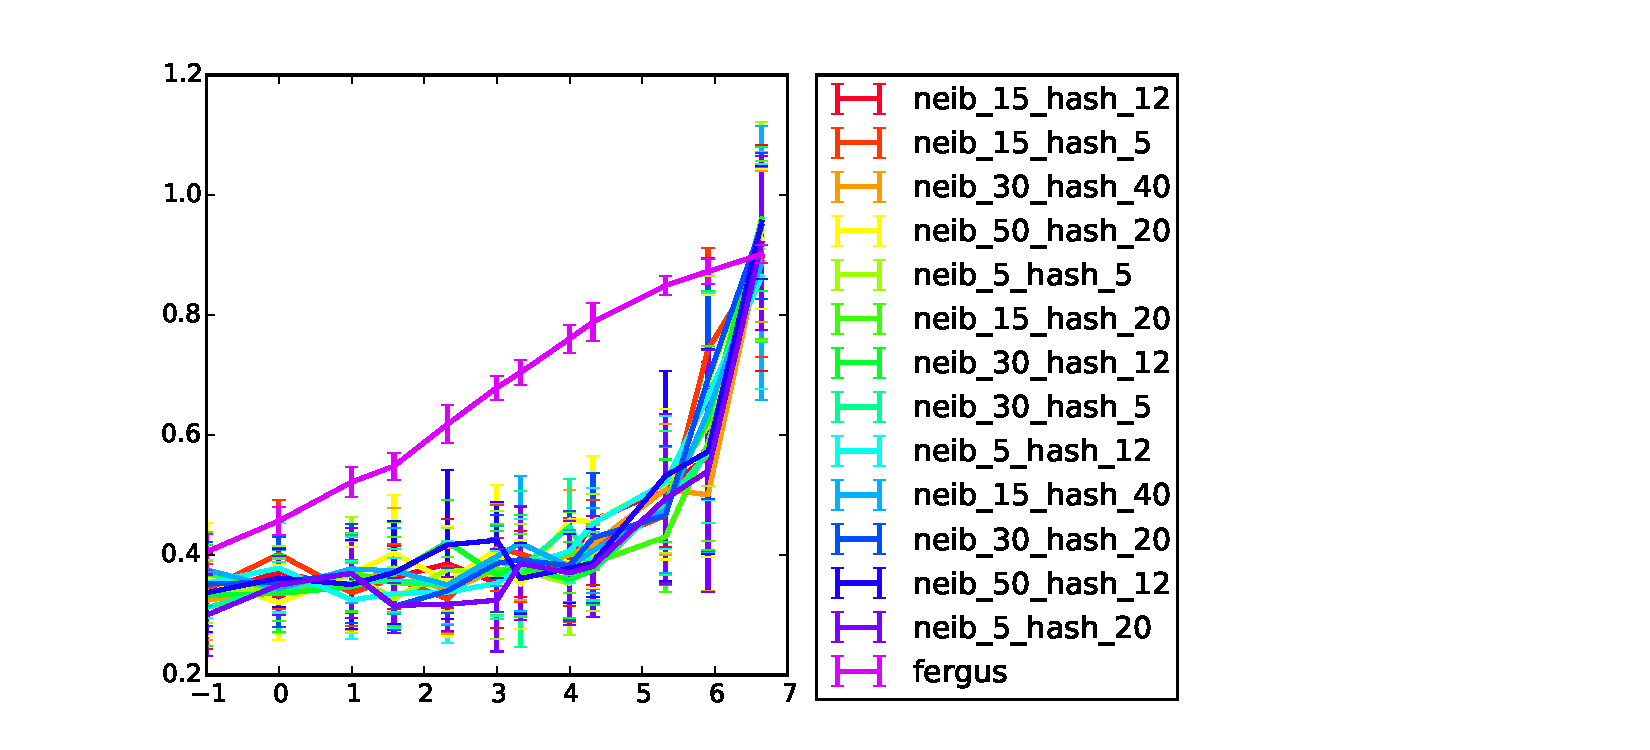
\includegraphics[width=\textwidth]{method_comp.pdf}
\end{figure}
\end{frame}

\section{Conclusion}
\begin{frame}{Conclusion}
\begin{itemize}
\item It seems plausible that the error term due to LSH is an $\mathcal{O}(n^{-1/2})$. But the bound is hard to obtain because of the many factors.
\item Computational limitations of our current implementation prevented us from proper testing of LSH+HFS methodology
\end{itemize}
\end{frame}

\begin{frame}{Future work}
\begin{itemize}
 
 \item Find sensible simplifications to allow bounding of the error term
 \item Check whether or not this error affect the underlying diffusion process estimation
 \item Evaluate other data-aware LSH methods and adapt the bounds
\end{itemize}
\end{frame}











\end{document}